\section{ELKStack}
\label{chapter:application:elkstack}

\textbf{ELKStack} - akronim opisujący stos technologi, składający się z 3 elementów:
\begin{itemize}
    \item[ElasticSearch] - pełnotekstowy silnik wyszukiwania,
    \item[Logstash] - scentralizowane przetwarzanie danych,
    \item[Kibana] - interfejs graficzny silnika \textbf{ElasticSearch}.
\end{itemize}

\subsection{Logstash}
    Logstash jest wysoce elastycznym narzędziem nie tylko w kontekście architektury \textbf{ELKStack}.
    Możliwe jest skonfigurowanie go w taki sposób, aby działał jako kolektor danych lub jako ich filtr czy też
    transformator. Składa się on z 3 elementów:
    \begin{itemize}
        \item sekcji wejścia,
        \item sekcji przetwarzania,
        \item sekcji wyjścia.
    \end{itemize}
    Każda z nich może składać się z więcej niż jednego bloku opisującego jej zadania.
    Innymi słowy ilość wejść jest nieograniczona, tak samo jak możliwości przetwarzania
    odbieranych danych oraz ostatecznie wysłania ich do więcej niż jednej lokalizacji.
    Ponadto dla każdej z nich możliwe jest napisanie własnego modułu lub wykorzystanie
    jednego z ciągle rosnącej listy publicznie dostępnych.
    
    Jest to ponadto rozwiązanie szybkie oraz łatwo skalowalne. Uruchomienie kolejnej
    instancji sprowadza się do przygotowania odpowiedniego pliku konfiguracyjnego
    i dostarczenia go jako argumentu wejściowego do pliku wykonywalnego aplikacji Logstash.
    Dzięki ciągle rozbudowywanej bazie wtyczek potrafi on jednak o wiele więcej. 
    Rozszerzenia można podzielić na 3 grupy, które odpowiadają omówionym wyżej sekcjom.
    Możliwe jest wybranie dowolnego rodzaju źródła danych, nie musi być nim wcale plik fizyczny.
    Logstash może także czytać z kolejek takich jak Kafka, bazy danych lub socket'ów.
    W sekcji przetwarzania można umieścić logikę odpowiedzialną za dodawanie, usuwanie poszczególnych
    pól. Możliwe jest także umieszczenie w środku małego programu napisanego w języku Ruby, jeśli oczywiście
    jest to konieczne. Ostatecznie ilość obsługiwanych wyjść można zacząć opisywać od innego
    elementu stosu technologicznego jakim jest \textbf{ELKStack}, czyli samej bazy danych
    \textbf{ElasticSearch}, a zakończyć na wypisywaniu kolejnych wydarzeń na konsolę. 

\subsection{ElasticSearch}
\label{chapter:application:elkstack:elasticsearch}
    \textbf{ElasticSearch} to pełnotekstowy, indeksowany silnik wyszukiwania. Jednak jest on także
    nierelacyjną bazą danych opartą o koncepcję dokumentów. Możliwość przechowywania oraz wyszukiwania
    informacji pośród zgromadzonych danych, które mogą mieć zarówno ustaloną, jak i luźną strukturę jest
    szczególnie istotna dla zarządzania logami. Tym, co wyróżnia każdy z nich jest informacja, wiadomość
    zawarta w kolejnych rekordach, a która jest inna w każdym przypadku. 
    
    ElasticSearch, dzięki indeksacji, oferuje możliwość pełnotekstowego wyszukiwania przechowywanych danych. Każda informacja, która wpływa do aplikacji, nie jest po prostu tam zapisywana.
    Specjalnie skonfigurowane indeksy pozwalają na określenie tego, co jest istotne. Ale nie jest
    to konieczne. Jedną z wartych wspomnienia funkcji tego narzędzia jest automatyczna detekcja typów danych, osiągana za pomocą samych danych. Wspomniane indeksy są tworzone automatycznie, aby jak najszybciej można było
    wykorzystać możliwości oferowane przez \textbf{ElasticSearch}.
    
    \textbf{Multitenancy} to cecha, wyróżnik chmur obliczeniowych. Jest ona bardzo łatwa do osiągnięcia
    dzięki grupowaniu i indeksacji w \textbf{ElasticSearch}. Grupa idealnie oddaje koncepcję tenanta.
    Wszystkie dane dla niego zgromadzone mogą zostać odszukane poprzez wskazania indeksu. Jest on
    tożsamy z grupą, a w dalszej kolejności tenantem.
    
    Jest to także rozwiązanie łatwo skalowalne. \textbf{ElasticSearch} posiada ten mechanizm wbudowany.
    Innymi słowy każda nowo uruchomiana instancja poszukuje w sieci, w której działa, innych instancji
    samoistnie budując klaster złożony z lidera oraz replik. 
    Lider odpowiedzialny jest za koordynację pracy klastra i może również przechowywać dane.
    Repliki stanowią odzwierciedlenie stanu lidera. Jeśli którakolwiek z instancji zostanie wyłączona z klastra, będzie
    potrafiła się samodzielnie przebudować. Dane przesyłane są między replikami. Ostatecznie uzyskuje się
    stan równowagi. Utracenie lidera nie stanowi przeszkody dla poprawnego działania, ponieważ pozostałe maszyny 
    "wynegocjują" wybór nowego lidera i całość będzie ponownie gotowa do świadczenia pełnej funkcjonalności w relatywnie
    krótkim czasie.
    
    \begin{figure}[h]
        \centering
        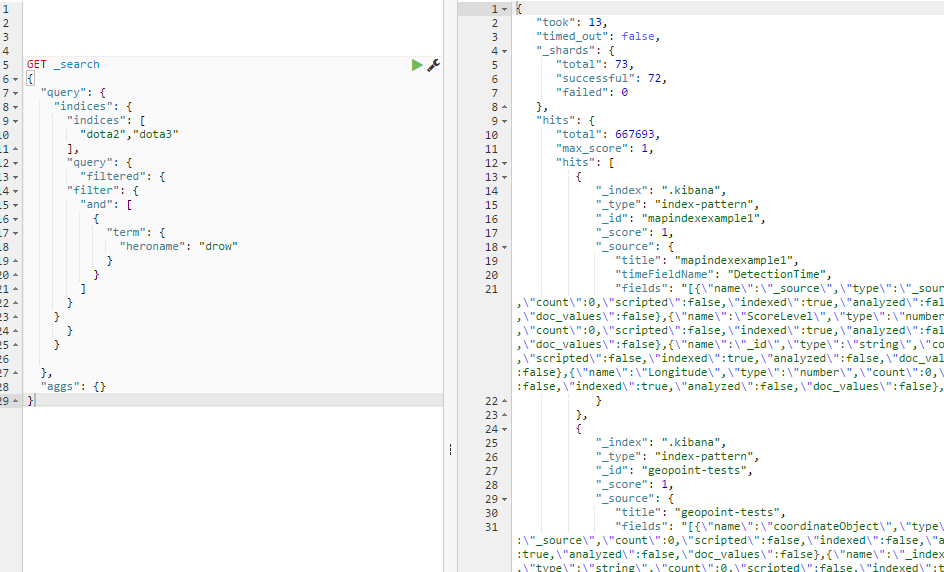
\includegraphics[width=1.0\textwidth]{images/es_query}
        \caption[Przykładowe zapytania do ElasticSearch]{
            Przykładowe zapytania do ElasticSearch, źródło: \url{http://i.stack.imgur.com/GFMUd.png}
        }
        \label{chapter:application:elkstack:es:query}
    \end{figure}
    
    Ostatecznie, i co szczególnie ważne, \textbf{ElasticSearch} oferuje całą funkcjonalność poprzez
    protokół HTTP. Znacznie upraszcza to proces administracyjny, ponieważ nie są wymagane żadne
    dodatkowe narzędzia. Niemniej, tworzenia tego typu aplikacji, jest również w znacznym stopniu uproszczone.
    Zakres operacji rozciąga się od zarządzania zawartością bazy danych, zgodnie z paradygmatem \textbf{CRUD}
    \footnote{\textbf{C}reate\textbf{R}ead\textbf{U}pdate\textbf{Delete} - skrót opisujące 4 podstawowe
        operacje, udostępnienie przez serwery WWW do zarządzania przechowywanymi na nich danymi.}, 
    aż do czynności takich jak:
    \begin{itemize}
        \item monitorowania stanu poszczególnej instancji lub całego klastra,
        \item manipulowanie ustawieniami szablonów dla przechowywanych dokumentów \cite{elastic_docs}.
    \end{itemize}

\clearpage

\subsection{Kibana}
\label{chapter:application:elkstack:kibana}

    \textbf{Kibana} to ostatni z elementów \textbf{ELKStack}. Jego zadaniem jest dostarczanie graficznego interfejsu
    użytkownika dla \textbf{ElasticSearch}. Z poziomu aplikacji dostępnej przez przeglądarkę możliwe
    jest przeglądanie wszystkich danych zgromadzonych przez \textbf{Logstash}, z użyciem tradycyjnych
    metod przeszukiwania, takich jak:
    \begin{itemize}
        \item filtrowanie,
        \item kwerendy, w tym wypadku pełnotekstowe.
    \end{itemize}
    
    Niemniej, to co jest szczególnie użyteczne to wizualizacja danych. Domyślny widok pozwala przeglądać 
    rekordy w formie zbliżonej do tabeli. 
    \begin{figure}[h]
        \centering
        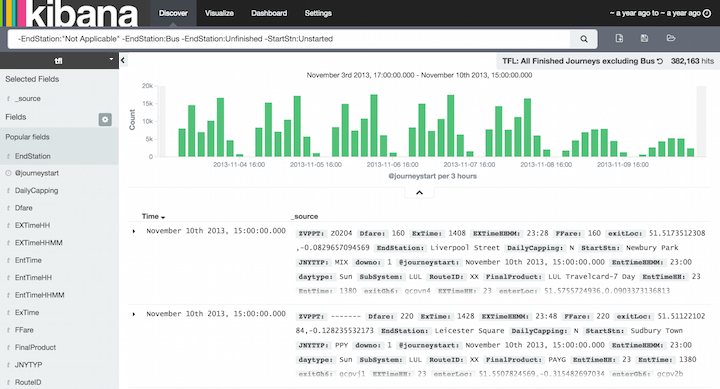
\includegraphics[width=1.0\textwidth]{images/kibana_main_view}
        \caption[Ekran główny w Kibana]{
            Ekran główny w Kibana, źródło: \url{https://www.elastic.co/guide/en/kibana/current/introduction.html}
        }
        \label{chapter:application:elkstack:kibana:main_view}
    \end{figure}
    W tym samym miejscu można zaobserwować jak Kibana współpracuje z ElasticSearch. Na rysunku \ref{chapter:application:elkstack:kibana:main_view} po lewej stronie widoczny jest pasek szybkiego
    wyszukiwania. Znajdujące się tam pozycje odpowiadają kolejnym właściwościom przeglądanego zbioru danych.
    Korzystając z niego, potencjalny użytkownik ma możliwość szybkiego filtrowania danych. Ilość filtrów jest
    nieograniczona. Ważnym jest, że nawet przy włączeniu wszystkich dostępnych filtrów, użytkownik w dalszym ciągu, może napisać
    własne zapytania \textbf{QueryDSL} i przesłać je do serwera. Kibana domyślnie sortuje dane w kolejności
    rosnącej względem skonfigurowanego pola dla danego indeksu. Rekordy można oglądać w dowolnym wycinku czasu.
    
    Szczególnie interesującą cechą wyników wyszukiwań, które można przeglądać w Kibana, jest to, że bezproblemowo
    łączą się one z dowolną formą wizualizacji. I tak samo, jak użytkownik, mógłby chcieć przejrzeć dane 
    jedynie z konkretnych dwóch godzin, konkretnego dnia, tak samo, możliwe jest uruchomienie podobnego
    filtru dla wykresu kołowego lub słupkowego.
    \begin{figure}[H]
        \centering
        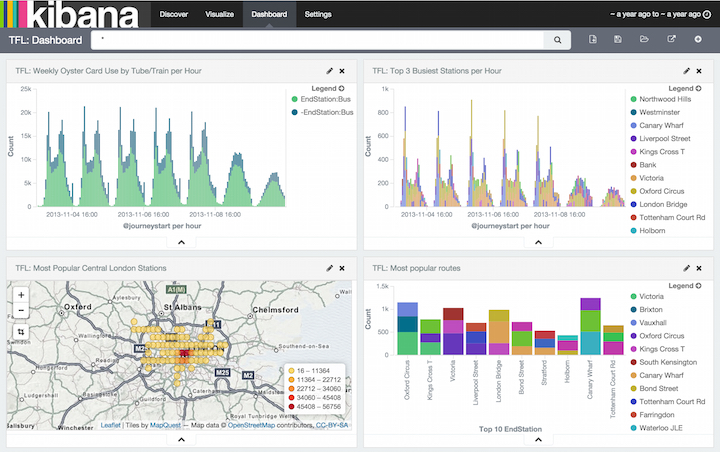
\includegraphics[width=1.0\textwidth]{images/kibana_dashboards}
        \caption[Ekran współdzielony w Kibana]{
            Ekran współdzielony w Kibana, źródło: \url{https://www.elastic.co/guide/en/kibana/current/introduction.html}
        }
        \label{chapter:application:elkstack:kibana:dashboard}
    \end{figure}
    Wykresy te w dalszym ciągu można łączyć w tak zwane \textbf{dashboards}, które stanowią idealne narzędzia do kolaboracji
    w tym samym zespole. Prócz tego, że pozwalają one na pokazanie jednocześnie więcej niż jednej wizualizacji, z których
    każda odnosi się do tego samego momentu w czasie, da się je zapisywać i przekazywać innym członkom zespołu. 